\documentclass[
a4paper,                        % paper size
11pt,                           % font size
twoside,                        % two sided
footsepline,                    % add a line to separate the footer
headsepline,                    % add a line to separate the header
headexclude,                    % header does not belong to the text
footexclude,                    % footer does not belong to the text
pagesize,                       % set the pagesize in a DVI document
bibtotocnumbered,               % add the bibliography to the TOC
idxtotoc                        % add the index to the TOC
%openright,                      % start a new chapter on the right page
%,DIV12
%,draft
]{scrreprt}

\usepackage{nameref}            % nameref, varioref, hyperref must be
                                % used in this order (see hyperref
                                % README)!
\usepackage[draft]{varioref}    % defines \vref
\usepackage{hyperref}           % automatically creates links when
                                % using pdflatex, defines \url
\usepackage{ifpdf}              % defines \ifpdf
\usepackage{graphicx}           % handles graphics
\usepackage{makeidx}            % creates the index
\usepackage{fancybox}

%%%%%%%%%%%%%%%%%%%%%%%%%%%%%%%%%%%%%%%%%%%%%%%%%%
%%%%%%%%%%%%%%%%%%%%%%%%%%%%%%%%%%%%%%%%%%%%%%%%%%
%%%%%%%%% New Commands and Environments %%%%%%%%%%
%%%%%%%%%%%%%%%%%%%%%%%%%%%%%%%%%%%%%%%%%%%%%%%%%%
%%%%%%%%%%%%%%%%%%%%%%%%%%%%%%%%%%%%%%%%%%%%%%%%%%
\newcommand{\es}{\textsf{ESPResSo}}
\newcommand{\ie}{\textit{i.e.\/}}
\newcommand{\eg}{\textit{e.g.\/}}
\newcommand{\etal}{\textit{et al.\/}}

\newcommand{\variant}[2]{(#1) \texttt{#2}\\}
%\newcommand{\lit}[1]{\texttt{#1}}
\newcommand{\var}[1]{\textrm{\textit{#1}}}
\newenvironment{syntax}{%
  \begin{Sbox}
    \begin{minipage}{0.9\linewidth}
    }{%
    \end{minipage}
  \end{Sbox}
  \begin{center}
    \fbox{\TheSbox}
  \end{center}
}

%%%%%%%%%%%%%%%%%%%%%%%%%%%%%%%%%%%%%%%%%%%%%%%%%%
%%%%%%%%%%%%%%%%%%%%%%%%%%%%%%%%%%%%%%%%%%%%%%%%%%
%%%%%%%%%%%%%%%% Other Settings %%%%%%%%%%%%%%%%%%
%%%%%%%%%%%%%%%%%%%%%%%%%%%%%%%%%%%%%%%%%%%%%%%%%%
%%%%%%%%%%%%%%%%%%%%%%%%%%%%%%%%%%%%%%%%%%%%%%%%%%
\pagestyle{headings}
\makeindex

%%%%%%%%%%%%%%%%%%%%%%%%%%%%%%%%%%%%%%%%%%%%%%%%%%
%%%%%%%%%%%%%%%%%%%%%%%%%%%%%%%%%%%%%%%%%%%%%%%%%%
%%%%%%%%%%%%%%%%% Main Document %%%%%%%%%%%%%%%%%%
%%%%%%%%%%%%%%%%%%%%%%%%%%%%%%%%%%%%%%%%%%%%%%%%%%
%%%%%%%%%%%%%%%%%%%%%%%%%%%%%%%%%%%%%%%%%%%%%%%%%%
\begin{document}
\titlehead{
  \begin{center}
    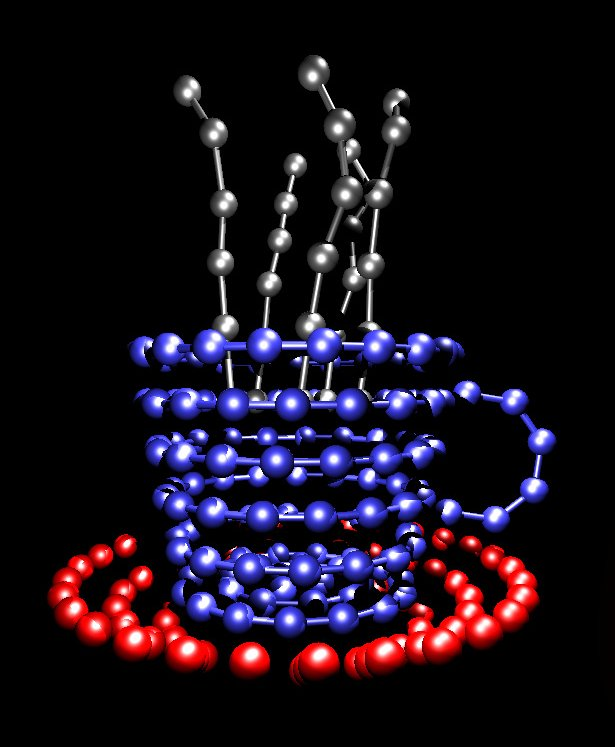
\includegraphics[width=5cm]{logo.jpg}
  \end{center}
}
%\subject{}
\title{\es{} User's Guide}
%\author{}
%\date{\today}
\maketitle

\tableofcontents

\chapter{Introduction}
\label{chap:intro}

\todo{Make the following lists full text.}

\begin{itemize}
\item \es{} is a generic soft matter simulation packages
\item for molecular dynamics simulations in soft matter research
\item focussed on coarse-grained models
\item employs modern algorithms (Lattice-Boltzmann, DPD, P3M, \ldots)
\item written in C for maximal portability
\item Tcl-controlled
\item parallelized
\end{itemize}

\section{Guiding principles}
\label{sec:ideas}

(from paper: 2.1 Goals and principles)

\es
\begin{itemize}
\item does \emph{not} do the physics for you!
\item requires you to understand what you do (can not be used as a
  black box)
\item gives you maximal freedom (flexibility)
\item is extensible
\item integrates system setup, simulation and analysis, as this can't
  be strictly separated in soft matter simulations
\item has no predefined units
\item sets as few defaults as possible
\end{itemize}

\section{Algorithms contained in \es}

The following algorithms are implemented in \es{}:

\begin{itemize}
\item ensembles: NVE, NVT, NpT
\item charged systems:
  \begin{itemize}
  \item P3M for fully periodic systems
  \item ELC and MMM-family of algorithms for charged systems with
    non-periodic boundary conditions
  \item Maggs algorithm 
  \end{itemize}
\item Hydrodynamics:
  \begin{itemize}
  \item DPD (as a thermostat)
  \item Lattice-Boltzmann
  \end{itemize}
\end{itemize}

\section{Basic program structure}
\label{sec:structure}

(from paper: 2.2 Basic program structure)

\begin{itemize}
\item Control level: \texttt{Tcl}
\item ``Kernel'' written in \texttt{C}
\item This user's guide will focus on the control level
\end{itemize}

\section{On units}
\label{sec:units}
\index{units}
\index{length unit}
\index{time unit}
\index{energy unit}
\index{physical units}

What is probably one of the most confusing subjects for beginners of
\es is, that \es does not predefine any units.  While most MD programs
specify a set of units, like, for example, that all lengths are
measured in \AA ngstr\"om or nanometers, times are measured in nano- or
picoseconds and energies are measured in $\frac{kJ}{\mathrm{mol}}$,
\es does not do so.

Instead, the length-, time- and energy scales can be freely chosen by
the user.  A length of $1.0$ can mean a nanometer, an \AA ngstr\"om,
or a kilometer - depending on the physical system, that the user has
in mind when he writes his \es-script.  The user can choose the unit
system that suits the system best.

When creating particles that are intended to represent a specific type
of atoms, one will probably use a length scale of \AA ngstr\"om.  This
would mean, that \eg the parameter $\sigma$ of the Lennard-Jones
interaction between two atoms would be set to twice the van-der-Waals
radius of the atom in \AA ngstr\"om.  Alternatively, one could set
$\sigma$ to $2.0$ and measure all lengths in multiples of the
van-der-Waals radius.

The second choice to be made is the energy (and time-) scale.  One can
for example choose to set the Lennard-Jones parameter $\epsilon$ to
the energy in $\frac{kJ}{\mathrm{mol}}$.  Then all energies will be
measured in that unit.  Alternatively, one can choose to set it to
$1.0$ and measure everything in multiples of the van-der-Waals binding
energy.

As long as one remains within the same unit system throughout the
whole \es-script, there should be no problems.

\section{Requirements}
\label{sec:requirements}
\index{requirements}

The following libraries and tools are required to be able to compile
and use \es:

\begin{description}
\item[Tcl/Tk] \index{Tcl/Tk} \es{} requires the Toolkit Command
  Language Tcl/Tk \footnote{\url{http://www.tcl.tk/}} in the version
  8.3 or later.  Some example scripts will only work with Tcl 8.4. You
  do not only need the interpreter, but also the header files and
  libraries.  Depending on the operating system, these may come in
  separate development packages. If you want to use a graphical user
  interface (GUI) for your simulation scripts, you will also need Tk.
  
\item[FFTW] \index{FFTW} In addition, \es{} needs the FFTW library
  \footnote{\url{http://www.fftw.org/}} for Fourier transforms.
  ESPResSo can work with both the 2.1.x and 3.0.x series. Again, the
  header files are required.
  
\item[MPI] \index{MPI} Finally, if you want to use \es{} in parallel,
  you need a working MPI environment (version 1.2). Currently, the
  following MPI implementations are supported:
  \begin{itemize}
  \item LAM/MPI is the preferred variant
  \item MPICH, which seems to be considerably slower than LAM/MPI in
    our benchmarks.
  \item On AIX systems, \es{} can also use the native POE parallel
    environment.
  \item On DEC/Compaq/HP OSF/Tru64, \es{} can also use the native
    dmpirun MPI environment.
  \end{itemize}
\end{description}


\section{Syntax description}
\label{sec:syntax}


Throughout the user's guide, formal definitions of the syntax of
several Tcl-commands can be found. The following conventions are used
in these decriptions:
\begin{itemize}
\item Different \emph{variants} of a command are labelled \variant{1},
  \variant{2}, \ldots
\item Keywords and literals of the command that have to be typed
  exactly as given are written in \lit{typewriter} font.
\item If the command has variable arguments, they are set in
  \var{italic font}. The description following the syntax definition
  should contain a detailed explanation of the argument and its
  type.
\item \texttt{\alt{\var{alt1} \asep \var{alt2}}} specifies, that one
  of the alternatives \var{alt1} or \var{alt2} can be used.
\item \texttt{\opt{\var{argument}}} specifies, that the arugment
  \var{argument} is optional, \ie{} it can be omitted.
\item When an optional argument or a whole command is marked by a
  superscript label (\fmark{1}), this denotes that the argument can
  only be used, when the corresponding feature (see appendix
  \vref{chap:features}) specified in ``Required features'' is
  activated.
\end{itemize}


\minisec{Example}

\renewcommand{\variant}[1]{\par\rawvariant{#1}}
\begin{essyntaxbox}
  \variant{1} 
  constraint wall normal \var{n_x} \var{n_y} \var{n_z} 
  dist \var{d} type \var{id}
  
  \variant{2}
  constraint sphere center \var{c_x} \var{c_y} \var{c_z} 
  radius \var{rad} direction \var{direction} type \var{id} 
  
  \require{1}{%
    \variant{3}
    constraint rod center \var{c_x} \var{c_y} 
    lambda \var{lambda}
  } 
  
  \require{2,3}{%
    \variant{4}
    constraint ext_magn_field \var{f_x} \var{f_y} \var{f_z} 
  }

  \begin{features}
    \required{CONSTRAINTS}
    \required[1]{ELECTROSTATICS}
    \required[2]{ROTATION}
    \required[3]{DIPOLES}
  \end{features}

\end{essyntaxbox}
\renewcommand{\variant}[1]{\rawvariant{#1}}

%%% Local Variables: 
%%% mode: latex
%%% TeX-master: "ug"
%%% End: 

\chapter{Tutorial}
\label{chap:tutorial}

\section{Quick installation}

\index{configure}\index{make}

If you have the requirements (see section \vref{sec:requirements})
installed, in many cases, to compile \es{}, it is enough to execute
the following sequence of two steps in the directory where you have
unpacked the sources:
\begin{verbatim}
> configure
> make
\end{verbatim}

In some cases, \eg{} when \es{} needs to be compiled for several
different platforms or when different versions with different sets of
features are required, it might be useful to execute the commands not
in the source directory itself, but to start \texttt{configure} from
another directory (see section \vref{sec:builddir}). Furthermore, many
features of \es{} can be selectively turned on or off in the local
configuration header of \es{} (see section \vref{sec:myconfig}) before
starting the compilation with \texttt{make}.

The shell script \texttt{configure} prepares the source code for
compilation. It will determine how to use and where to find the
different libraries and tools required by the compilation process, and
it will test what compiler flags are to be used.  The script will find
out most of these things automatically.  If something is missing, it
will complain and give hints how to solve the problem.  The
configuration process can be controlled with the help of a number of
options that are explained in section \vref{sec:configure}.

The command \texttt{make} will compile the source code. Depending on
the options passed to the program, \texttt{make} can also be used for
a number of other things:
\begin{itemize}
\item It can install and uninstall the program to some other
  directories. However, normally it is not necessary to actually
  \textit{install} \es{} to run it.
\item It can test the \es{} program for correctness.
\item It can build the documentation.
\end{itemize}
The details of the usage of \texttt{make} are described in section
\vref{sec:make}.

When these steps have successfully completed, \es{} can be started
with the command (see section \vref{sec:run})
\begin{verbatim}
> Espresso
\end{verbatim}

\section{Running \es{}}
\begin{itemize}
\item Do we need that?
\item interactive use (sample session) ?really advertise that?
\item small sample session ????
\item script execution (see below)
\end{itemize}

\section{Doing a simulation}

\es{} is implemented as an extension to the Tcl script language. This means that you need to write a
script for any task you want to perform with \es. To learn about the Tcl script language and
especially the \es{} extensions, this chapter offers two tutorial scripts. The first will guide you
step by step through creating your first simulation script, while the second script is a well
documented example simulation script. Since the latter is slightly more complex and uses more
advanced features of \es{}, we recommend to work through both scripts in the presented order.

\subsection{Creating your first simulation script}

This section introduces some of the features of \es\ by
constructing step by step a simulation script for a simple salt crystal.
We cannot give a full Tcl tutorial here; however, most of the constructs
should be self--explanatory. We also assume that the reader is familiar with the
basic concepts of a MD simulation here. The code pieces can be copied step by
step into a file, which then can be run using \verb|Espresso <file>| from the
\es{} source directory.

Our script starts with setting up the initial configuration.  Most conveniently,
one would like to specify the density and the number of particles of the system
as parameters:
\begin{verbatim}
set n_part 200; set density 0.7
set box_l [expr pow($n_part/$density,1./3.)]
\end{verbatim}
These variables do not change anything in the simulation engine, but are just
standard Tcl variables; they are used to increase the readability and
flexibility of the script. The box length is not a parameter of this simulation;
it is calculated from the number of particles and the system density. This
allows to change the parameters later easily, e.~g.\ to simulate a bigger
system.

The parameters of the simulation engine are modified by the \verb|setmd|
command. For example
\begin{verbatim}
setmd box_l $box_l $box_l $box_l
setmd periodic 1 1 1
\end{verbatim}
defines a cubic simulation box of size \verb|box_l|, and periodic boundary
conditions in all spatial dimensions. We now fill this simulation box with
particles
\begin{verbatim}
set q 1; set type 0
for {set i 0} { $i < $n_part } {incr i} {
  set posx [expr $box_l*[t_random]]
  set posy [expr $box_l*[t_random]]
  set posz [expr $box_l*[t_random]]
  set q [expr -$q]; set type [expr 1-$type]
  part $i pos $posx $posy $posz q $q type $type }
\end{verbatim}
This loop adds \verb|n_part| particles at random positions, one by one.  In this
construct, only two commands are not standard Tcl commands: the random
number generator \verb|t_random| and the \verb|part| command, which is used to
specify particle properties, here the position, the charge \verb|q| and the
type. In \es\ the particle type is just an integer number which allows to group
particles; it does not imply any physical parameters. Here we use it to tag the
charges: positive charges have type 0, negative charges have type 1.

Now we define the ensemble that we will be simulating. This is done using the
\verb|thermostat| command. We also set some integration scheme parameters:
\begin{verbatim}
setmd time_step 0.01; setmd skin 0.4
set temp 1; set gamma 1
thermostat langevin $temp $gamma
\end{verbatim}
This switches on the Langevin thermostat for the NVT ensemble, with temperature
\verb|temp| and friction \verb|gamma|. The skin depth \verb|skin| is a parameter
for the link--cell system which tunes its performance, but cannot be discussed
here.

Before we can really start the simulation, we have to specify the interactions
between our particles.  We use a simple, purely repulsive Lennard-Jones
interaction to model the hard core repulsion \cite{grest86a}, and the charges interact via the
Coulomb potential:
\begin{verbatim}
set sig 1.0; set cut   [expr 1.12246*$sig]
set eps 1.0; set shift [expr 0.25*$eps]
inter 0 0 lennard-jones $eps $sig $cut $shift 0
inter 1 0 lennard-jones $eps $sig $cut $shift 0
inter 1 1 lennard-jones $eps $sig $cut $shift 0
inter coulomb 10.0 p3m tunev2 accuracy 1e-3 mesh 32
\end{verbatim}
The first three \verb|inter| commands instruct \es\ to use the same purely
repulsive Lennard--Jones potential for the interaction between all combinations
of the two particle types 0 and 1; by using different parameters for different
combinations, one could simulate differently sized particles.  The last line sets
the Bjerrum length to the value 10, and then
instructs \es\ to use P$^3$M for the Coulombic interaction and to try to find
suitable parameters for an rms force error below $10^{-4}$, with a fixed mesh
size of 32. The mesh is fixed here to speed up the tuning; for a real
simulation, one will also tune this parameter.

Now we can integrate the system:
\begin{verbatim}
set integ_steps 200
for {set i 0} { $i < 20 } { incr i} {
  set temp [expr [analyze energy kinetic]/(1.5*$n_part)]
  puts "t=[setmd time] E=[analyze energy total], T=$temp"
  integrate $integ_steps }
\end{verbatim}
This code block is the primary simulation loop and runs
$20\times$\verb|integ_steps| MD steps. Every \verb|integ_steps| time steps, the
potential, electrostatic and kinetic energies are printed out (the latter one as
temperature). However, the simulation will crash: \es\ complains about particle
coordinates being out of range. The reason for this is simple: Due to the
initial random setup, the overlap energy is around a million kT, which we first
have to remove from the system. In \es, this is can be accelerated by capping
the forces, i.~e.\ modifying the Lennard--Jones force such that it is constant
below a certain distance. Before the integration loop, we therefore insert this
equilibration loop:
\begin{verbatim}
for {set cap 20} {$cap < 200} {incr cap 20} {
  puts "t=[setmd time] E=[analyze energy total]"
  inter ljforcecap $cap; integrate $integ_steps }
inter ljforcecap 0
\end{verbatim}
This loop integrates the system with a force cap of initially 20 and finally
200.  The last command switches the force cap off again. With this
equilibration, the simulation script runs fine.

However, it takes some time to simulate the system, and one will probably like
to write out simulation data to configuration files, for later analysis. For
this purpose \es\ has commands to write simulation data to a Tcl stream
in an easily parsable form.  We add the following lines at end of integration
loop to write the configuration files ``config\_0'' through ``config\_19'':
\begin{verbatim}
  set f [open "config_$i" "w"]
  blockfile $f write tclvariable {box_l density}
  blockfile $f write particles {id pos type}
  close $f
\end{verbatim}
The created files ``config\_...'' are human--readable and look like
{\footnotesize
\begin{verbatim}
{tclvariable
        {box_l 10}
        {density 0.7}
}
{particles {id pos type}
        {0 3.51770181433 4.3208975936 5.30529948918 0}
        {1 3.93145531704 6.58506447035 6.95045147034 1}
        ...
}
\end{verbatim}}
As you can see, such a \emph{blockfile} consists of several Tcl lists,
which are called \emph{blocks}, and can store any data available from the
simulation. Reading a configuration is done by the following simple script:
\begin{verbatim}
set f [open $filename "r"]
while { [blockfile $f read auto] != "eof" } {}
close $f
\end{verbatim}
The \verb|blockfile read auto| commands will set the Tcl variables \verb|box_l| and
\verb|density| to the values specified in the file when encountering the \verb|tclvariable| block,
and the particle positions and types of all 216 particles are restored when the \verb|particles|
block is read.

\begin{figure}[tb]
  \centering
  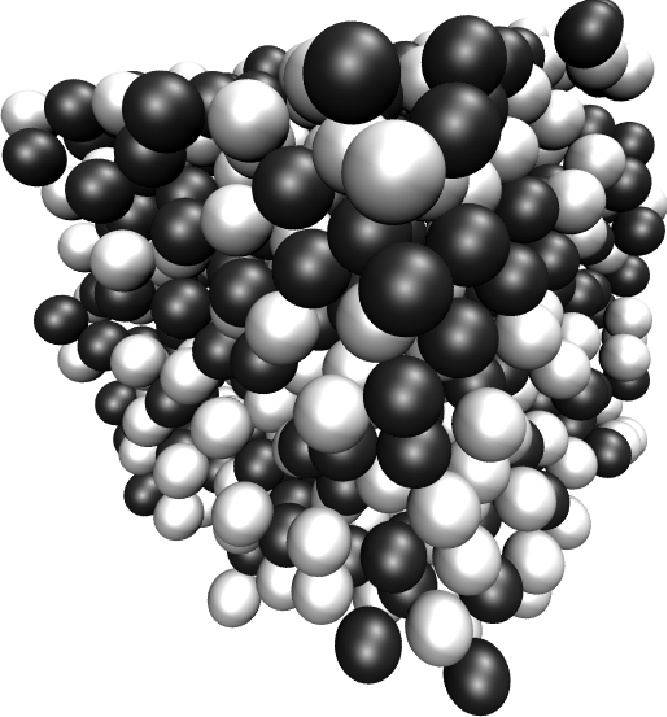
\includegraphics[width=0.4\textwidth]{figures/salt.png}
  \caption{VMD Snapshot of the salt system}
  \label{fig:snapshot}
\end{figure}

With these configurations, we can now investigate the system. As an example, we
will create a second script which calculates the averaged radial distribution
functions $g_{++}(r)$ and $g_{+-}(r)$. The radial distribution function for a
the current configuration can be obtained using the \verb|analyze| command:
\begin{verbatim}
set rdf [analyze rdf 0 1 0.9 [expr $box_l/2] 100]
foreach value [lindex $rdf 1] {
  lappend rlist   [lindex $value 0]
  lappend rdflist [lindex $value 1] }
\end{verbatim}
The shown \verb|analyze rdf| command returns the distribution function of
particles of type 1 around particles of type 0 (i.~e.\ of opposite charges) for
radii between $0.9$ and half the box length, subdivided into $100$ bins.
Changing the first two parameters to either ``0 0'' or ``1 1'' allows to
determine the distribution for equal charges. The result is a list of $r$ and
$g(r)$ pairs, which the following foreach loop divides up onto two lists
\verb|rlist| and \verb|rdflist|.

To average over a set of configurations, we put the two last code snippets into
a loop like this:
\begin{verbatim}
set cnt 0
for {set i 0} {$i < 100} {incr i} { lappend avg_rdf 0}
foreach filename $argv {
  set f [open $filename "r"]
  while { [blockfile $f read auto] != "eof" } {}
  close $f
  set rdf [analyze rdf 0 1 0.9 [expr $box_l/2] 100]
  foreach value [lindex $rdf 1] {
     lappend rlist   [lindex $value 0]
     lappend rdflist [lindex $value 1] }
  set avg_rdf [vecadd $avg_rdf $rdflist]
  incr cnt }
set avg_rdf [vecscale [expr 1/$cnt] $avg_rdf]
\end{verbatim}
Initially, the sum of all $g(r)$, which is stored in \verb|avg_rdf|, is set to
0.  Then the loops over all configurations given by \verb|argv|, calculates
$g(r)$ for each configuration and adds up all the $g(r)$ in \verb|avg_rdf|.
Finally, this sum is normalized by dividing by the number of configurations.
Note that \verb|argv| is a predefined variable: it contains all the command line
parameters. Therefore this analyzation script should be called like\\
\verb|Espresso <script> <config 1> <config 2> ...|. 

\begin{figure}[tb]
  \centering
  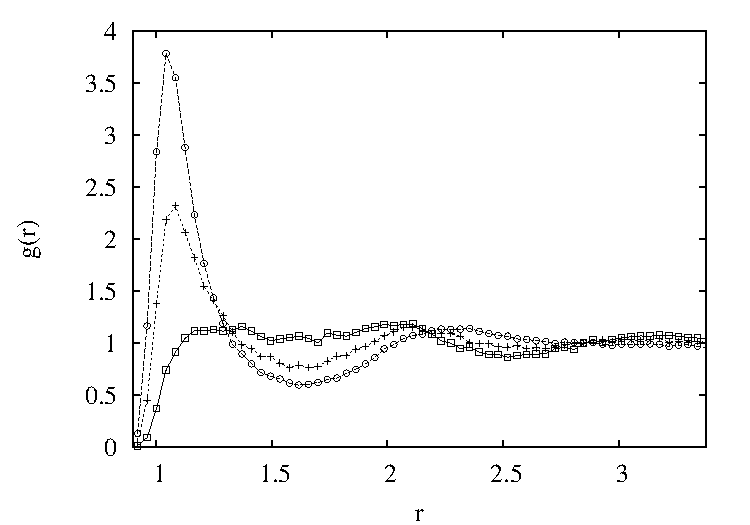
\includegraphics[width=0.7\textwidth]{figures/nacl-rdf.pdf}
  \caption{Radial distribution functions $g_{++}(r)$ between equal charges
    (rectangles) and $g_{+-}(r)$ for opposite charges (circles). The plus
    symbols denote $g(r)$ for an uncharged system.}
  \label{fig:rdf}
\end{figure}

The printing of the calculated radial distribution functions is simple. Add to the end of the
previous snippet the following lines:
\begin{verbatim}
set plot [open "rdf.data" "w"]
puts $plot "\# r rdf(r)"
foreach r $rlist rdf $avg_rdf { puts $plot "$r $rdf" }
close $plot
\end{verbatim}
This instructs the Tcl interpreter to write the \verb|avg_rdf| to the file \verb|rdf.data| in
gnuplot--compatible format. Fig.~\ref{fig:rdf} shows the resulting radial distribution functions,
averaged over 100 configurations. In addition, the distribution for a neutral
system is given, which can be obtained from our simulation script by simply
removing the command \verb|inter coulomb ...| and therefore not turning on P$^3$M.

The code example given before is still quite simple, and the reader is
encouraged to try to extend the example a little bit, e.~g. by using differently
sized particle, or changing the interactions. If something does not work, \es\
will give comprehensive error messages, which should make it easy to identify
mistakes. For real simulations, the simulation scripts can extend over thousands
of lines of code and contain automated adaption of parameters or online
analysis, up to automatic generation of data plots.  Parameters can be changed
arbitrarily during the simulation process, as needed for e.~g.\ simulated
annealing. The possibility to perform non--standard simulations without the need
of modifications to the simulation core was one of the main reasons why we
decided to use a script language for controlling the simulation core.

\subsection{\texttt{tutorial.tcl}}

In the samples folder you will find a well documented simulation script \texttt{tutorial.tcl}, which
takes you step by step through a slightly more complicated simulation of a polyelectrolyte
system. The basic structure of the script is however the same as in the previous example and
probably the same as the structure of most \es{} simulation scripts.

Initially, some parameters and
global variables are set, the interactions are initialized, and particles are added. For this, the
script makes use of the \verb|polymer| command, which provides a faster way to set up chain
molecules.

The actual simulation falls apart again into two loops, the warmup loop with increasing force
capping, and the final simulation loop. Note that the electrostatic interaction is only activated
after equilibrating the excluded volume interactions, which speeds up the warmup phase. However,
depending on the problem, this splitted warmup may not be possible due to physical
restrictions. \es{} cannot detect these mistakes and it is your responsibility to find simulation
procedure suitable to your specific problem.

%%% Local Variables: 
%%% mode: latex
%%% TeX-master: "ug"
%%% End: 

\chapter{Compiling and installing \es}
\label{chap:install}
\index{Installation|textbf}

\begin{itemize}
\item Compiling \es{} is a necessary evil
\item Features can be compiled in or not
\item For maximal efficiency, compile in only the features that you
  use
\item \es{} can be obtained from the \es{} home page
  \footnote{\url{http://www.espresso.mpg.de}}.
\item If you are looking for the \es binary or the object files, read
  \vref{sec:builddir}
\item other than in most packages, \es will probably not be installed,
  or it will only be installed locally. Refer to \vref{sec:installdir}
  for details.
\end{itemize}

\section{Source and build directories}
\label{sec:builddir}
\index{build directory} \index{source directory}

Usually, when a program is compiled, the resulting binary files are
put into the same directory as the sources of the program. In \es, the
\emph{source directory} that contains all the source files is
completely separated from the \emph{build directory} where the files
created by the build process are put. As the source directory is not
modified during the compilation process, it is possible to compile more
than one binary versions of \es from a single set of source files.

The location of the build directory is determined when
\texttt{configure} is called.  Depending on whether it is called from
the source directory where it resides, or from some other directory,
the build system will act different.

When \texttt{configure} is called from another current working
directory than the source directory, this directory will become the
\emph{build directory}.  All files will be generated below the build
directory.  This way, you can make as many builds of \es as you like,
each build having different compiler flags and built-in features, and
for as many platforms as you want.  All further commands concerning
compiling and running \es{} have to be called from this directory,
instead of from the source directory.

When \texttt{configure} is called from the source directory where the
script resides, the \es build system has limited built-in capabilities
to handle different computer hardware.  A new subdirectory is created
in the source directory and \texttt{configure} is recursively called
from this directory, making the subdirectory the build directory.  The
directory is called \texttt{obj-}\textit{platform}\texttt{/}, where
\textit{platform} is an automatically determined descriptor of the CPU
type where the script was started, \eg
\mbox{\texttt{obj-Athlon\_64-pc-linux}}.  Note that this heuristic
will work in many cases, but it may not always work as intended.  When
you notice any problems, you can always call \texttt{configure} from
another directory.

In this case it is also possible to run the commands \texttt{make} and
\texttt{Espresso} directly in the source directory.  Furthermore, the
option \texttt{--enable-chooser} will be set in the recursive call of
\texttt{configure} that activates the automatic binary chooser (see
section \vref{sec:installdir}).

\paragraph{Example}
When the source directory is \texttt{\$srcdir} (\ie{} the files where
unpacked to this directory), then the build directory can be set to
\texttt{\$builddir} by calling the \texttt{configure}-script from
there:
\begin{code}
cd $builddir
$srcdir/configure
make
Espresso
\end{code}

\section{\texttt{myconfig.h}: Activating and deactivating features}
\label{sec:myconfig}

\index{features} \index{myconfig.h} \index{configuration header} \es
has a large number of features that can be compiled into the binary.
However, it is not recommended to actually compile in all possible
features, as this will negatively affect \es's performance.  Instead,
compile in only the features that are actually required.  For the
developers, it is also possible to turn on or off a number of
debugging messages.  The features and debug messages can be controlled
via a configuration header file that contains C-preprocessor
declarations. Appendix \vref{chap:features} lists and describes all
available features.  When no configuration header is provided by the
user, a default header will be used that turns on the default
features.  The file \texttt{myconfig-sample.h} in the source directory
contains a list of all possible features that can be copied into your
own configuration file.

When you distinguish between the build and the source directory (see
\vref{sec:builddir}), the configuration header can be put in either of
these. Note, however, that when a configuration header is found in
both directories, the one in the build directory will be used.  For an
example how this can be employed, see section \ref{sec:builddir}.

By default, the configuration header is called \texttt{myconfig.h}.
The name of the configuration header can be changed either when the
\texttt{configure}-script is called with the option
\mbox{\texttt{--with-myconfig}} (see section \vref{sec:configure}), or
when \texttt{make} is called with the setting
\mbox{\texttt{myconfig=}\textit{myconfig\_header}} (see section
\vref{sec:make}).

The configuration header can be used to compile different binary
versions of \es with a different set of features from the same source
directory.  Suppose that you have a source directory \texttt{\$srcdir}
and two build directories \texttt{\$builddir1} and
\texttt{\$builddir2} that contain different configuration headers:

\begin{itemize}
\item \texttt{\$builddir1/myconfig.h}:
\begin{code}
#define ELECTROSTATICS
#define LENNARD-JONES
\end{code}

\item \texttt{\$builddir2/myconfig.h}:
\begin{code}
#define LJCOS
\end{code}
\end{itemize}

\noindent Then you can simply compile two different versions of \es via
\begin{code}
cd $builddir1
$srcdir/configure
make

cd $builddir2
$srcdir/configure
make
\end{code}


\section{Running \texttt{configure}}
\label{sec:configure}

% Description of basic options: --prefix, --exec-prefix, CPPFLAGS,
% CFLAGS, LDFLAGS

\index{configure} The shell script \texttt{configure} collects all the
information required by the compilation process. It will determine how
to use and where to find the different libraries and tools required by
the compilation process, and it will test what compiler flags are to
be used.  The script will find out most of these things automatically.
If something is missing, it will complain and give hints how to solve
the problem.  The generic syntax of calling the \texttt{configure}
script is:
\begin{code}
configure [\var{options} ...] [\var{variable}=\var{value} ...]
\end{code}

\noindent Note that in the \es build system, the files generated by
the configuration and compilation process are not placed next to the
source files, but into a separate \emph{build directory} instead.
Refer to section \vref{sec:builddir} for details.

\index{configure options} The behaviour of \texttt{configure} can be
controlled by the means of command line options. In the following,
only those command line options that are specific to \es will be
explained.  For a complete list of options and explanations thereof,
call
\begin{code}
configure --help
\end{code}

\subsection{Options}

\begin{description}
\item [\texttt{--enable-chooser}] This option will enable the
  automatic binary chooser mechanism for \es (see section
  \vref{sec:installdir}).  This option will be automatically enabled,
  when the \texttt{configure} script is called from the source
  directory, otherwise it will be disabled. It is not recommended to
  set the option manually.
\item[\texttt{--enable-debug}] This option will enable compiler flags
  required for debugging the \es binary and is disabled by default.
\item[\texttt{--enable-profiling}] This option will enable compiler
  flags required for profiling the \es binary and is disabled by
  default.
\item[\texttt{--disable-processor-optimization}] This option will
  control whether \texttt{configure} will check for several
  optimization flags to be used by the compiler. This option is
  enabled by default.
\item[\texttt{--disable-xlc-qipa}] This option is only useful when the
  IBM C-compiler \texttt{xlc} is used and will control whether or not
  the compiler flag \texttt{-qipa} is used.  If you come upon problems
  when using the \es binary on IBM machines, try using
  \texttt{--disable-xlc-ipa}. The option is enabled by default.
\item[\texttt{--with-myconfig=MYCONFIG\_HEADER}] This option sets the
  name of the local configuration header (see \vref{sec:myconfig}). It
  defaults to ``\texttt{myconfig.h}''.
\item[\texttt{--with-mpi=MPI}/ \texttt{--without-mpi}] Sets the MPI
  implementation that should be used, or disables MPI. By default,
  \texttt{configure} will test automatically what MPI implementation
  is available. The following implementations are known:
  \begin{description}
  \item[\texttt{fake}, \texttt{no}] This will disable MPI
    completely. Equivalent to \mbox{\texttt{--without-mpi}}.
  \item[\texttt{lam}] Use the LAM/MPI environment
    (\url{http://www.lam-mpi.org/}).
  \item[\texttt{mpich}] Use the MPICH environment
    (\url{http://www-unix.mcs.anl.gov/mpi/mpich/}).
  \item[\texttt{poe}] Use the POE environment (IBM).
  \item[\texttt{dmpi}] Use the DMPI environment (Tru64).
  \item[\texttt{generic}] Use a generic MPI implementation. This will
    try to find an MPI compiler and an MPI runtime environment.
  \end{description}
\item[\texttt{--with-efence} / \texttt{--without-efence}] Whether or
  not to use the ``electric fence'' memory debugging library
  (\url{http://freshmeat.net/projects/efence/}). Efence is not used by
  default.
\item[\texttt{--with-tcl=TCL}] By default, \texttt{configure} will
  automatically determine which version of Tcl is used.  If the wrong
  version is chosen automatically, you can specify the name of the
  library with this option, \eg{} \texttt{tcl8.4}.
\item[\texttt{--with-tk=TK} / \texttt{--without-tk}] By default, the
  GUI toolkit Tk is not used by \es. This option can be used to
  activate Tk and to specify which Tk version to use, \eg{}
  \texttt{tk8.4}. If you only specify \texttt{--with-tk} and do not
  give a version number, \texttt{configure} will try to automatically
  deduce the right version.
\item[\texttt{--with-fftw=VERSION} / \texttt{--without-fftw}] This can
  be used to specify whether the FFTW library is to be used, and which
  version.  By default, version 3 will be used if it is found,
  otherwise version 2 is used.  Note that quite a number of central
  features of \es require FFTW.
\end{description}

\section{\texttt{make}: Compiling,  testing and installing \es}
\label{sec:make}

The command \texttt{make} is mainly used to compile the \es{} source
code, but it can do a number of other things. The generic syntax of
the \texttt{make} command is:
\begin{code}
make [\var{target}...] [\var{variable}=\var{value}]
\end{code}
When no target is given, the target \texttt{all} is used. The
following targets are available:
\begin{description}
\item[\texttt{all}] Compiles the complete \es source code. The
  variable \lit{myconf} can be used to specify the name of the
  configuration header to be used.
\item[\texttt{check}] Runs the testsuite. By default, all available
  tests will be run on 1, 2, 3, 4, 6, or 8 processors. Which tests are
  run can be controlled by means of the variable \texttt{tests}, which
  processor numbers are to be used can be controlled via the variable
  \texttt{processors}. Note that depending on your MPI installation,
  MPI jobs can only be run in the queueing system, so that \es{} will
  not run from the command line. In that case, you may not be able to
  run the testsuite, or you have to directly submit the testsuite script
  \verb!testsuite/test.sh! to the queueing system.\\
  \textbf{Example:} \verb!make check tests="madelung.tcl" processors="1 2"!\\
  will run the test \texttt{madlung.tcl} on one and two processors.
\item[\texttt{clean}] Deletes all files that were created during the
  compilation.
\item[\texttt{mostlyclean}] Deletes most files that were created
  during the compilation. Will keep for example the built doxygen
  documentation and the \es{} binary.
\item[\texttt{dist}] Creates a \texttt{.tar.gz}-file of the \es{}
  sources.  This will include all source files as they currently are
  in the source directory, \ie{} it will include local changes.  This
  is useful to give your version of \es{} to other people.
  The variable \texttt{extra} can be used to specify additional
  files and directories that are to be included in the archive
  file. \\
  \textbf{Example:} \verb!make dist extra="myconfig.h internal"!\\
  will create the archive file and include the file
  \texttt{myconfig.h} and the directory \texttt{internal} with all
  files and subdirectories.
\item[\texttt{install}] Install \es. The variables \texttt{prefix} and
  \texttt{exec-prefix} can be used to specify the installation
  directories, otherwise the defaults defined by the
  \texttt{configure} script are used. \texttt{prefix} sets the prefix
  where all \es files are to be installed, \texttt{exec-prefix} sets
  the prefix where the executable files are to be installed and is
  required only when there is an architecture-specific directory (\eg
  \texttt{/usr/local/bin64/}).  For the actual locations where the
  different files are installed, refer to section
  \vref{sec:installdir}.\\
  \textbf{Example:} \verb!make install prefix=/usr/local!\\
  will install all files below \texttt{/usr/local}.
\item[\texttt{uninstall}] Uninstalls \es{}, \ie{} removes all files
  that were installed during \texttt{make install}. The variables are
  identical to the variables of the \texttt{install}-target.
\end{description}

\subsection{Installation directories}
\label{sec:installdir}

\index{installation directory} Other than most software, \es is not
necessarily installed into the system, but can also be used directly
from the build directory.  The rest of this section is only
interesting if you plan to install \es.

Normally, the \es-binary \texttt{Espresso-bin} is installed in the
directory \texttt{\$prefix/libexec/} and a the wrapper script
\texttt{Espresso} in the directory \texttt{\$prefix/bin/} that handles
the MPI invocation.

When the \texttt{configure}-script is called from the source directory
or when the option \texttt{--enable-chooser} is given, an automatic
binary chooser is installed in the directory \texttt{\$prefix/bin/}
and the \es-binary and the MPI wrapper script are installed in an
architecture-specific subdirectory
\mbox{\texttt{\$exec-prefix/lib/espresso/obj-}\textit{platform}\texttt{/}}.
When called, the binary chooser will automatically call the MPI
wrapper script from the right subdirectory.

\section{Running \es}
\label{sec:run}

When \es is found in your path, it can be run via
\begin{code}
Espresso [\var{tcl\_script} [\var{N\_processors} [\var{args}]]]
\end{code}

\index{interactive mode} When \es{} is called without any arguments,
it is started in the interactive mode, where new commands can be
entered on the command line. When the name of a \textit{tcl\_script}
is given, the script is executed. \textit{N\_processors} is the number
of processors that are to be used. Any further arguments are passed to
the script. Note that depending on your MPI installation, MPI jobs can
only be run in the queueing system, so that \es will not run from
the command line.

% A number of wrapper scripts are used in running \es{}:
% \begin{itemize}
% \item The script \texttt{Espresso} in the source and build directory
%   will try to run the compiled version of \es. If it is called from
%   the source directory, it assumes that \es{} was also configured in
%   the source directory and will try to recursively start the script in
%   the corresponding \texttt{obj-PLATFORM} build directory. If it is
%   called in the build directory, it will start the \es-binary with the
%   right MPI implementation.
% \item The chooser script \texttt{Espresso} 
%   \begin{itemize}
%   \item installed when \verb!--enable-chooser! was given
%   \item installed to bindir
%   \item tries to run the correct version of the MPI-wrapper
%     \texttt{Espresso}
%   \end{itemize}
% \item The MPI-wrapper \texttt{Espresso}
%   \begin{itemize}
%   \item installed next to \es{} binary
%   \item starts the binary with the right MPI implementation
%   \end{itemize}
% \item The \es{} binary \texttt{Espresso-bin} can also be started
%   directly, however, it requires that the environment variable
%   \verb!ESPRESSO_SCRIPTS! is set to the directory where the scripts
%   are installed (usually \verb!$(prefix)/lib/espresso/scripts! or
%   \verb!$(prefix)/share/espresso/scripts!).
% \end{itemize}


%%% Local Variables: 
%%% mode: latex
%%% TeX-master: "ug"
%%% End: 

\chapter{\es{} command reference}
\label{chap:ref}

(most from paper and from related pages)

\begin{itemize}
\item Will contain description of all Tcl-commands
\item Reference to appendix \vref{chap:quickref}
\item basic identifiers:
  \begin{itemize}
  \item particle type
  \item bonded interaction type
  \item molecule id
  \end{itemize}
\end{itemize}


\section{\texttt{inter}: Setting up interactions}
\label{sec:inter}
\begin{command}
  \variant{1}
  {inter
    \var{part\_type\_id1} 
    \var{part\_type\_id2}
    \var{inter\_type} 
    [ \var{parameters}\ldots ]
  }
  \variant{2}
  {inter
    \var{bond\_type\_id} \var{bond\_type} [
    \var{parameters}\ldots ]
  }
  \variant{3}
  {inter}
\end{command}

\section{Writing VTF files}
There are two commands in \es{} that support writing files in the VMD
formats VTF, VSF and VCF.\footnote{A description of the format and a
  plugin to read the format in VMD is found in the subdirectory
  \texttt{vmdplugin/} of the \es{} source directory.} The commands can
be used to write the structure (\texttt{writevsf}) and coordinates
(\texttt{writevcf}) of the system to a single trajectory file (usually
with the extension \texttt{.vtf}), or to separate files (extensions
\texttt{.vsf} and \texttt{.vtf}).

\subsection{\texttt{writevsf}}

\begin{command}
  writevsf \var{file} \var{options}
\end{command}
Writes a structure block describing the system's structure to
\var{file}. The atom ids used in the file are identical to \es's
particle ids.  This makes it easy to write additional structure lines
to the file, e.g. to specify the \texttt{resname} of particle
compounds, like chains.  The output of this file can be used in a
standalone VSF file, or at the beginning of a trajectory VTF file that
contains a trajectory of a whole simulation.

\paragraph{Options}
\begin{options}
  short|verbose
\end{options}
Specify, whether the output is in a human-readable, but somewhat
longer format (\keyword{verbose}), or in a more compact form
(\keyword{short}). The default is \keyword{verbose}.

\begin{options}
  radius \var{radii}|auto
\end{options}
Specify the VDW radii of the atoms. \var{radii} is either
\keyword{auto}, or a Tcl-list describing the radii of the different
particle types. When the keyword \keyword{auto} is used and a
Lennard-Jones interaction between two particles of the given type is
defined, the radius is set to be $\frac{\sigma_{LJ}}{2}$ plus the LJ
shift.  Otherwise, the radius $0.5$ is substituted. The default is
\keyword{auto}.  

Example: \verb!radius {{0 2.0} {1 auto} {2 1.0}}!

\begin{options}
  typedesc \var{typedesc}
\end{options}
\var{typedesc} is a Tcl-list giving additional VTF atom-keywords to
specify additional VMD characteristics of the atoms of the given type.
If no description is given for a certain particle type, it defaults to
\texttt{segid \textit{n}}, where \textit{n} is the type id.

Example: \verb!typedesc {{0 "segid colloid"} {1 "segid pe"}}!


\subsection{\texttt{writevcf}}
\begin{command}
  writevcf \var{file} \var{options}
\end{command}
Writes a coordinate (or timestep) block that contains all coordinates
of the system's particles to \var{file}.

\paragraph{Options}
\begin{options}
  short|verbose
\end{options}
Specify, whether the output is in a human-readable, but somewhat
longer format (\keyword{verbose}), or in a more compact form
(\keyword{short}). The default is \keyword{verbose}.

\begin{options}
  folded|absolute
\end{options}
Specify whether the particle positions are written in absolute
coordinates (\keyword{absolute}) or folded into the central image of a
periodic system (\keyword{folded}). The default is \keyword{absolute}.

\begin{options}
  pids \var{pids}|all
\end{options}
Specify the coordinates of which particles should be written. If
\keyword{all} is used, all coordinates will be written (in the ordered
timestep format). Otherwise, \var{pids} has to be a Tcl-list
specifying the pids of the particles. The default is \keyword{all}.

Example: \verb!pids {0 23 42}!



    % \section{Creating particles}
% \label{sec:part}
% \texttt{part}

% \section{Interactions}
% \label{sec:inter}
% \texttt{inter}

% \section{Analysis}
% \label{sec:analysis}

%%% Local Variables: 
%%% mode: latex
%%% TeX-master: "ug"
%%% End: 

\chapter{Under the hood}
\label{chap:underhood}

(new)

\begin{itemize}
\item Implementation issues that are interesting for the user
\item Main loop in pseudo code (for comparison)
\item from doxygen: ``Cell systems'' 
\end{itemize}

%%% Local Variables: 
%%% mode: latex
%%% TeX-master: "ug"
%%% End: 

\chapter{Getting involved}
\label{chap:devel}

\begin{itemize}
\item What to do when you want to become involved
\item How to submit a bug report
\item Reference to developer's guide
\end{itemize}

%%% Local Variables: 
%%% mode: latex
%%% TeX-master: "ug"
%%% End: 


\appendix
\chapter{\es{} quick reference}
\label{chap:quickref}

\begin{itemize}
\item Short reference table of all commands
\item Complete syntax of \es{} commands
\item Features required for different commands
\end{itemize}

\chapter{The MMM family of algorithms}
\label{chap:mmm}

\chapter{Maggs algorithm}
\label{chap:maggs}

\printindex

\end{document}


%%% Local Variables: 
%%% mode: latex
%%% TeX-master: t
%%% End: 
